\PassOptionsToPackage{unicode}{hyperref}
\PassOptionsToPackage{hyphens}{url}
%
\documentclass[12pt, a4paper]{article}
\usepackage[a4paper,margin=1in]{geometry}
\setlength\parindent{0pt}
\usepackage{mathptmx}
\usepackage{amsmath,amssymb}
\usepackage[T1]{fontenc}
\usepackage[utf8]{inputenc}
\usepackage{textcomp}
\usepackage{comment}
\usepackage{hyperref}
\usepackage{graphicx}
\usepackage{float}
\usepackage{booktabs}
\usepackage{caption}

\author{Fabio Zanotti, Artificial Intelligence, ID number (matricola)
\\Edoardo Conca,  Artificial Intelligence ID number (matricola)
\\Antonio Morelli, Artificial Intelligence, ID number (matricola)}
\date{}
\title{International Trade Network Analysis: Understanding Global Economic Interactions}

\begin{document}
\maketitle

\section{Introduction}
\label{introduction}

International trade is the backbone of the global economy, enabling the exchange of goods, services, and resources between countries. The complex web of trade relationships influences not only national economies but also global economic stability and growth. Understanding these relationships is essential for policymakers, economists, and business leaders; network analysis offers a powerful means to unravel the intricacies of international trade.\\

Our work contributes to the field of economic network analysis, with a specific focus on identifying patterns, trends, and key players that shape global trade dynamics; to achieve this, we have adopted a \textit{Q\&A} format, in which we pose a series of questions and provide answers using appropriate measures to illuminate non-obvious relationships and outcomes.

\section{Problem and Motivation}
\label{problem-and-motivation}

Our work is motivated by the need to understand the characteristics of the infrastructure underlying the complex global trade network, particularly to determine whether a small group of powerful nations exerts disproportionate control over the flow of commodities. While posing and answering questions, we also seek to explore the nature of the countries involved in this network, investigating potential correlations between factors such as their type of government, their real \textit{GDP} (Gross Domestic Product), and the commodities they trade, which is vital for uncovering hidden dependencies in the global trade system.\\

A specific problem addressed by this network analysis is the identification of vulnerabilities within global trade networks. As global trade becomes increasingly interconnected, certain countries or trade routes may emerge as critical nodes or links. We wanted to determine what would be the impact on global trade and how worldwide economies would be affected if these critical points were to be disrupted—whether by geopolitical conflicts, natural disasters, or economic sanctions.

Therefore, understanding the dynamics of such a network is crucial for several reasons:
\begin{itemize}
    \item \textbf{Impact on National Economies}: Central countries in the trade network significantly influence trade flows and economic policies.
    \item \textbf{Global Economic Stability}: Insights into trade networks help predict and mitigate economic instability.
    \item \textbf{Policy Making}: Data-driven analysis aids in formulating effective economic policies.
\end{itemize}

The main contributions of our project include identifying key players and vulnerabilities in the global trade network, providing insights into the influence of political and economic factors.

\section{Datasets}
\label{datasets}

The \href{https://www.cia.gov/the-world-factbook/}{World Factbook} dataset provides basic intelligence on the history, people, government, economy, energy, geography, environment, communications, transportation, military, terrorism, and transnational issues for \textit{265} world entities, as collected by the \textit{CIA} (\textit{Central Intelligence Agency}).

The dataset is not directly offered in a format suitable for automatic analysis, so we initially considered performing web scraping from the official website; however, due to the high reputation of this dataset, we found an existing solution. The source code for this web scraping is available at this \href{https://github.com/lucafrance/cia-factbook-scraper}{link}, and the resulting \texttt{.json} file can be accessed on \href{https://www.kaggle.com/datasets/lucafrance/the-world-factbook-by-cia}{Kaggle}.

This file includes a plethora of information about 258 countries and entities involved in international trade. From the extensive list of available data, we selected the following fields:
\begin{itemize}
    \item \textbf{"Economy: Real GDP (purchasing power parity)"}: This field represents the total economic output of a country, adjusted for purchasing power parity (PPP). PPP is a method of measuring the relative value of currencies, which allows for a more accurate comparison of economic productivity and standards of living between countries by accounting for differences in price levels.

    \item \textbf{"Economy: Exports - partners"}: This field lists the countries or regions to which a country exports goods and services.

    \item \textbf{"Economy: Exports - commodities"}: This field details the main types of goods and services that a country exports.

    \item \textbf{"Economy: Imports - partners"}: This field specifies the countries or regions from which a country imports goods and services.

    \item \textbf{"Geography: Geographic coordinates"}: This field provides the latitude and longitude of a country or entity.

    \item \textbf{"Government: Government type"}: This field describes the form of government that a country has, such as a democracy, monarchy, or authoritarian regime.
    
\end{itemize}

Unfortunately, due to either errors in the scraping code or a complete absence of information, some smaller countries were missing one or more of these fields. Consequently, we decided to exclude these countries from our analysis, ending up with \textit{216} countries and \textit{1832} edges. We quickly noticed that the \textit{GDP} values referred to different years for each nation, which could undermine the accuracy of our outcomes; thankfully, the official \textit{Factbook} website offers the possibility to retrieve \href{https://www.cia.gov/the-world-factbook/references/guide-to-country-comparisons/}{official files} referring to \textit{2023} values, allowing us to ensure consistency when comparing numerical fields across countries.\\

% The excluded countries are:
% \textit{Akrotiri, Antarctica, Anguilla, Ashmore and Cartier Islands, Baker Island, Bouvet Island, British Indian Ocean Territory, Christmas Island, Clipperton Island, Cocos (Keeling) Islands, Coral Sea Islands, Dhekelia, French Southern and Antarctic Lands, Gaza Strip, Guernsey, Heard Island and McDonald Islands, Holy See (Vatican City), Howland Island, Isle of Man, Jan Mayen, Jarvis Island, Jersey, Johnston Atoll, Kingman Reef, Liechtenstein, Midway Islands, Navassa Island, Norfolk Island, Palmyra Atoll, Paracel Islands, Pitcairn Islands, Saint Barthelemy, Saint Helena, Ascension, and Tristan da Cunha, Saint Martin, Saint Pierre and Miquelon, Spratly Islands, Svalbard, Wake Island, Wallis and Futuna, West Bank, World}\\

The data underwent a cleaning process to remove unwanted characters, ensuring that the values were in a usable format. Trade partners for both exports and imports, as well as commodities, were extracted from their respective strings and converted into lists, while geographic coordinates were converted to decimal format for plotting. To enhance the analysis, we decided to change the taxonomy used for government types and commodities, aggregating the values into broader macrocategories. This standardization was guided by insights from law and political science students for government types, and by using the \textit{SITC} (\textit{Standard International Trade Classification}), a comprehensive method for categorizing traded goods, for commodities. The resulting dictionary was then converted into a \texttt{Pandas} dataframe.\\

\begin{table}[h]
\centering
\small
\scalebox{0.8}{%
\begin{tabular}{lllll}
\toprule
& \multicolumn{2}{c}{Before Cleaning} & \multicolumn{2}{c}{After Cleaning} \\
\cmidrule(lr){2-3} \cmidrule(lr){4-5}
& Government Types & Commodities & Government Types & Commodities \\
\midrule
Count & 51 & boh  & 19 & Ariboh   \\
\bottomrule
\end{tabular}
}
\captionsetup{font=scriptsize,labelfont=bf}
\caption{Comparison of categorical fields before and after cleaning.}
\label{tab:network_stats}
\end{table}

A graph was constructed using \texttt{Networkx}, a Python package for the creation, manipulation, and study of complex networks. The graph is directed and has a node for each country, with an edge indicating that "country x exports to country y." Edges were constructed using either the "Economy: Exports - partners" or the "Economy: Imports - partners" fields, with the latter orientation being reversed (i.e., if country x imports from country y, then country y exports to country x). For each pair of nodes, there can be a maximum of two edges, one going from the first to the second node and one in the opposite direction.

\begin{figure}[ht]
\centering
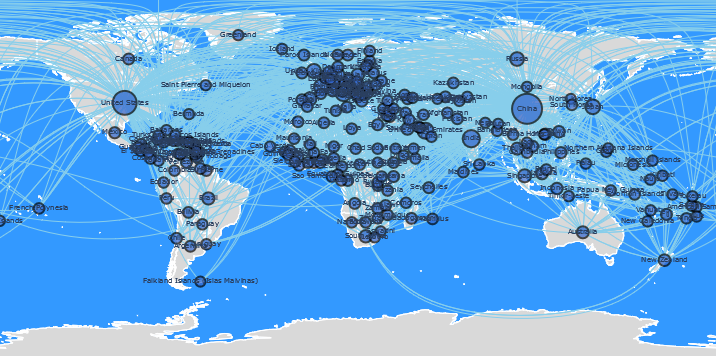
\includegraphics[width=.9\textwidth]{figures/question1/figure_1.png}
\captionsetup{font=scriptsize,labelfont=bf}
\caption{Network overview, node size coded by degree centrality.}
\label{fig:figure1}
\end{figure}

\section{Validity and Reliability}
\label{validity-and-reliability-not-needed-for-the-project-proposal}

The model we constructed aims to closely represent the reality of global trade networks by incorporating verified and comprehensive data from the US government. However, the validity of our model is influenced by certain limitations: the variation in the years of \textit{GDP} data across different countries posed a challenge to maintaining accuracy. We mitigated this by sourcing \textit{GDP} data consistently from 2023, ensuring better comparability.\\

Reliability in our study is maintained by following a standardized and step by step documented data-cleaning process; by clearly documenting the way we handle missing data and the standardization of categories, we have aimed to be as transparent as possible, ensuring that our study can be reproduced by others with similar results.\\

It is important to note that the data we use is publicly available and free to use, as stated in the official copyright notice:
\begin{quote}
The Factbook is in the public domain. Accordingly, it may be copied freely without permission of the Central Intelligence Agency (CIA). The official seal of the CIA, however, may NOT be copied without permission as required by the CIA Act of 1949 (50 U.S.C. section 403m). Misuse of the official seal of the CIA could result in civil and criminal penalties. \textit{About The World Factbook - Copyright and Contributors}
\end{quote}

\section{Measures and Results}
\label{measures}

We will construct this section following the same approach used to conduct the experiments. Therefore, we will pose a question, select one or more measures to answer it, explain the measure and its interpretation in our network and, finally, discuss the results.

\subsection{Which kind of countries play a major role in trade flow and which do not?}

The first question we explored concerns the nature of our nodes, which are the countries. Specifically, we sought to determine which countries are the most influential and which are not; we considered it interesting to examine the types of governments these countries have.

\subsubsection{Degree Centrality}

Degree centrality measures the number of direct connections a node has. In our context, it indicates the number of trade partners a country has. An incident connection for a node represents an import relationship, while a non-incident connection represents an export relationship. A higher degree centrality means that a country has more direct trade relationships, suggesting its central role in the network.\\

\begin{figure}[!ht]
\centering
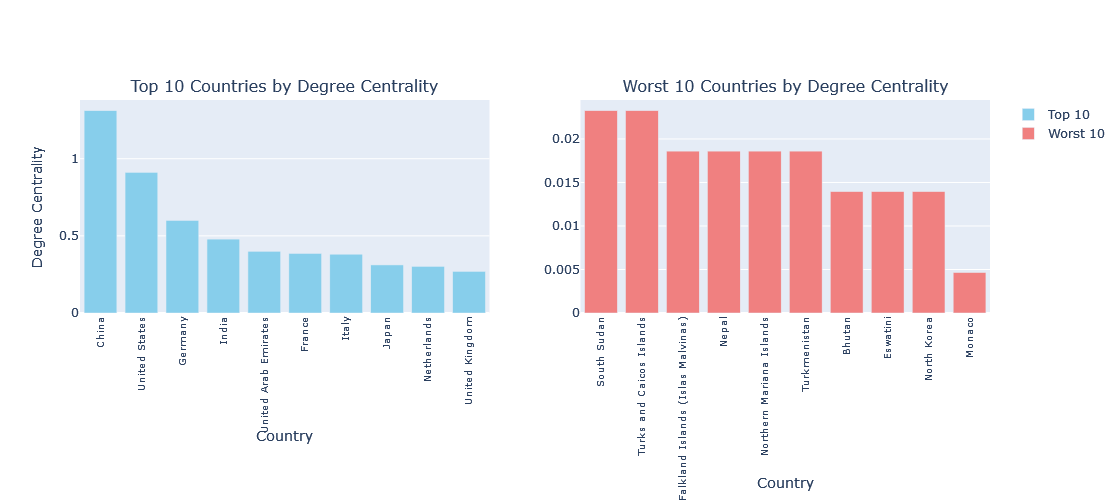
\includegraphics[width=\textwidth]{figures/question1/figure_2a.png}
\vspace{1em}
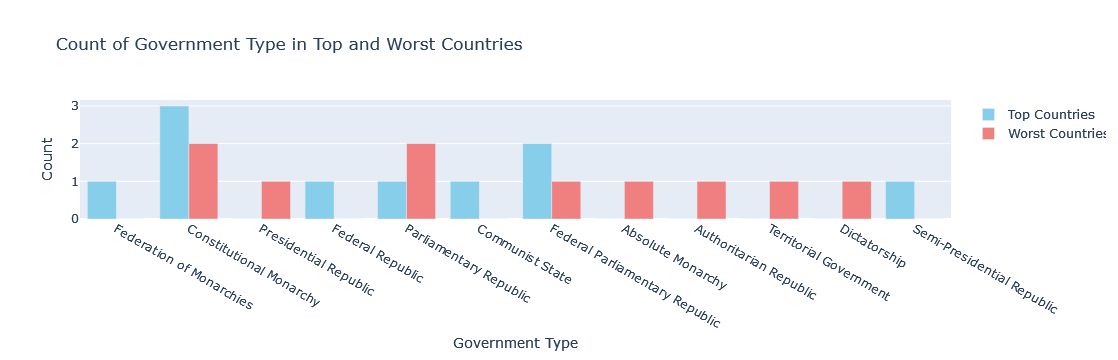
\includegraphics[width=\textwidth]{figures/question1/figure_2b.png}
\captionsetup{font=scriptsize,labelfont=bf}
\caption{Top and worst 10 countries by degree centrality (top) and their government types (bottom).}
\label{fig:figure2}
\end{figure}

% \begin{figure}[!ht]
% \centering
% 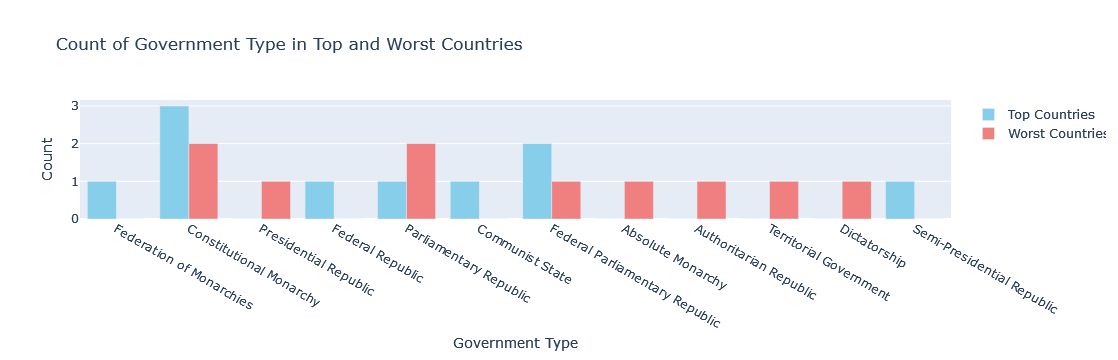
\includegraphics[scale=0.4]{figures/question1/figure_2b.png}
% \vspace{1em}
% \captionsetup{font=scriptsize,labelfont=bf}
% \caption{Government types of top and worst 10 countries by degree centrality.}
% \label{fig:figure2b}
% \end{figure}

The analysis of the top \textit{10} and worst \textit{10} countries by degree centrality \textit{(Figure 2)} in the trade network reveals some intriguing patterns related to government types and global economic integration. The countries with the highest centrality are predominantly democracies, including federal republics like the \textbf{United States} and \textbf{Germany}, as well as parliamentary systems such as those found in \textbf{Japan}, the \textbf{UK}, and much of the \textbf{European Union}. This suggests that democratic governance, often associated with open markets and strong international ties, tends to correlate with higher trade centrality. Interestingly, many of the top countries belong to the European Union, indicating that regional economic integration, along with shared governance standards, might also play a significant role in boosting trade centrality. In contrast, the countries with the lowest centrality often have more authoritarian or hybrid regimes, such as \textbf{North Korea}, \textbf{Turkmenistan}, and \textbf{Eswatini}, which are typically more isolated from global trade networks. Additionally, smaller nations or those with challenging economic conditions, like \textbf{Nepal} or \textbf{South Sudan}, also appear at the bottom, reinforcing the idea that both governance and economic development are critical factors in global trade positioning.\\

\begin{figure}[!ht]
\centering
% 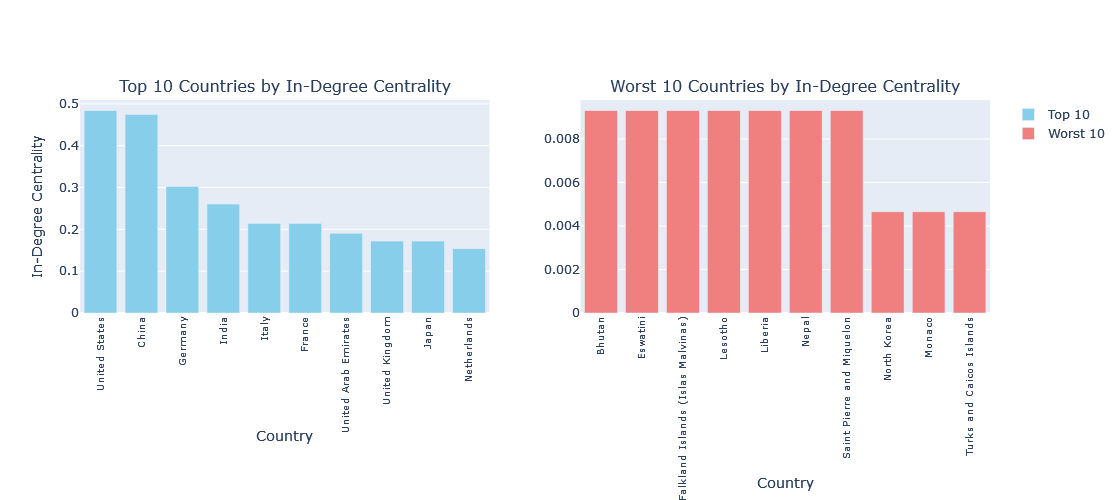
\includegraphics[width=\textwidth]{figures/question1/figure_3b.png}
% 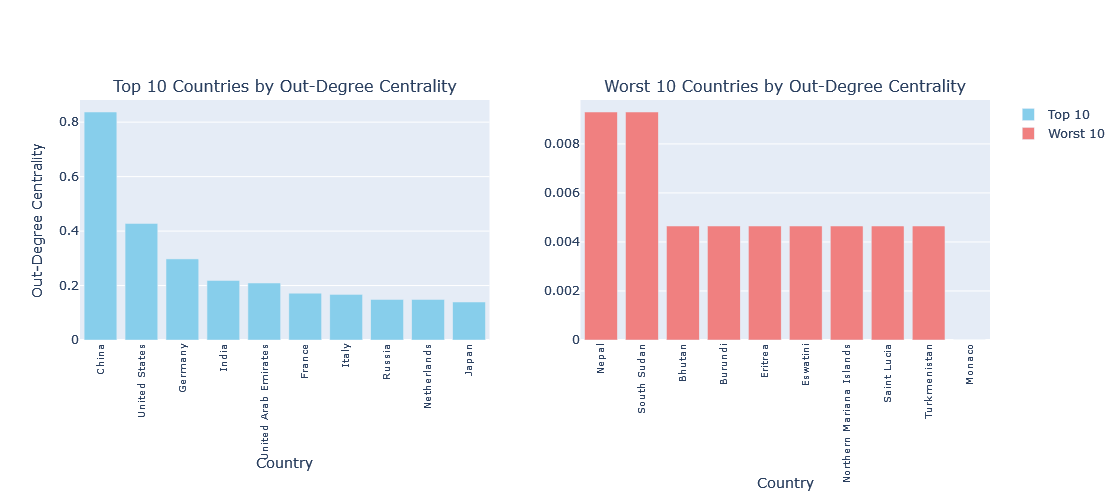
\includegraphics[width=\textwidth]{figures/question1/figure_3a.png}
\begin{minipage}[b]{0.45\textwidth}
    \centering
    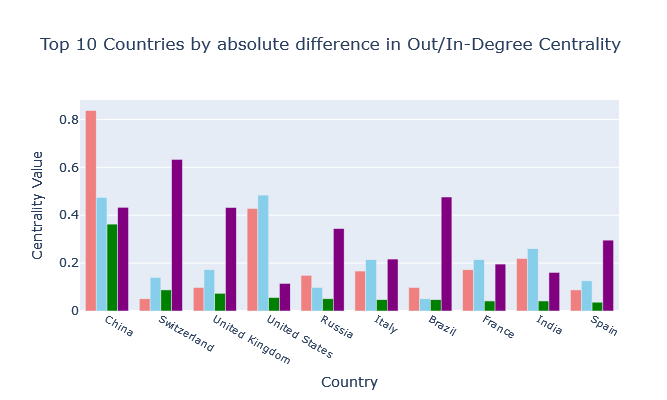
\includegraphics[width=\textwidth]{figures/question1/figure_3c.png}
\end{minipage}
\hfill
\begin{minipage}[b]{0.535\textwidth}
    \centering
    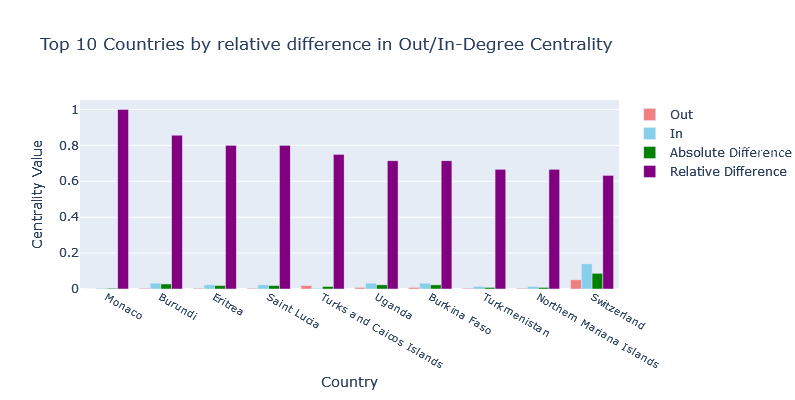
\includegraphics[width=\textwidth]{figures/question1/figure_3d.png}
\end{minipage}
\captionsetup{font=scriptsize,labelfont=bf}
\caption{Highest absolute (left) and relative (right) differences between out and in degree centralities.}
\label{fig:figure3}
\end{figure}

\textit{Figure 3} instead shows, respectively, the countries with the highest absolute and relative differences between in-degree and out-degree centralities. The first plot highlights the countries with the most significant absolute differences. Notably, \textbf{China} exhibits a substantial out-degree centrality, indicating its prominent role as a global exporter. This aligns with China's well-known position as the "world's factory," supplying a wide array of goods to markets across the globe. However, its relatively lower in-degree centrality reflects China's strategic efforts to reduce dependency on imports, further emphasizing its self-reliance in key sectors. \textbf{Switzerland} presents an interesting case with a relatively high difference between its out-degree and in-degree centrality. This discrepancy may be attributed to Switzerland's strong export-driven economy, particularly in high-value sectors like pharmaceuticals, machinery, and financial services, while it imports less in comparison.\\

The second plot sheds light on countries with the highest relative differences in out-degree and in-degree centrality. Interestingly, many of the countries listed here are smaller or less economically dominant on the global stage, such as \textbf{Burundi}, \textbf{Eritrea}, and \textbf{Saint Lucia}. These high relative differences are likely a result of their unique economic circumstances. Small countries often have high import centrality due to their need to import essential goods that cannot be produced domestically. Conversely, some small nations may exhibit high out-degree centrality due to niche exports or due to political and economic strategies aimed at self-sufficiency or specialization in specific industries. \textbf{Switzerland} again appears in this list, albeit this time for its high relative difference, reinforcing its unique position as a country that maintains a substantial export volume relative to its import needs.

\subsection{Is the trade flow mostly controlled by a few countries?}
\subsubsection{Degree Centrality Distribution}

The \textit{Degree Centrality Distribution} is crucial for understanding the connectivity pattern within a trade network. Fitting this distribution to a power law can reveal whether the network has a scale-free structure, characterized by a few highly connected nodes and many nodes with fewer connections. This is significant because it indicates the presence of dominant countries that act as major trade hubs, which can have substantial implications for network resilience, trade flow efficiency, and economic influence.

\begin{figure}[ht]
\centering
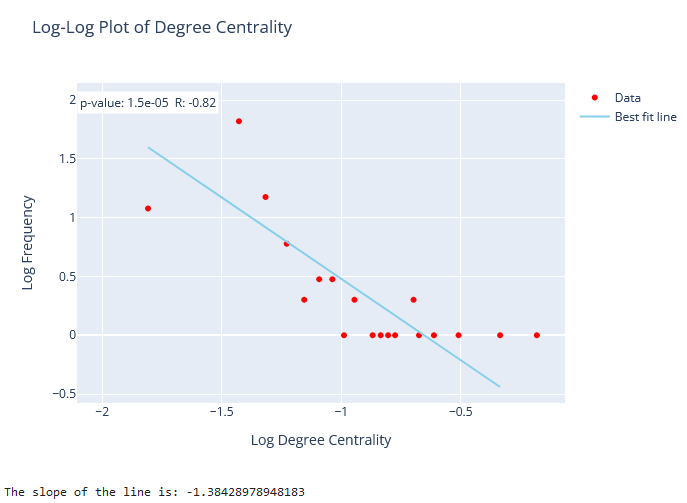
\includegraphics[width=.5\textwidth]{figures/question2/figure_4.png}
\captionsetup{font=scriptsize,labelfont=bf}
\caption{Degree centrality distribution. The slope of the line is \textit{-1.38428978948183}.}
\label{fig:figure4}
\end{figure}

The negativity as well as the consistently high absolute value of the fitted line in \textit{Figure 4}, suggest that just a few nodes of our network are highly connected, while the majority of them entertains commercial relationships with just a few countries.

\subsubsection{Cumulative Distribution for Degree Centrality}

The \textit{Cumulative Distribution for Degree Centrality} provides a complementary perspective by showing the proportion of countries with a degree centrality greater than or equal to a certain value. This plot helps to emphasize the tail of the distribution, making it easier to identify the presence and significance of highly connected countries within the trade network.

\begin{figure}[ht]
\centering
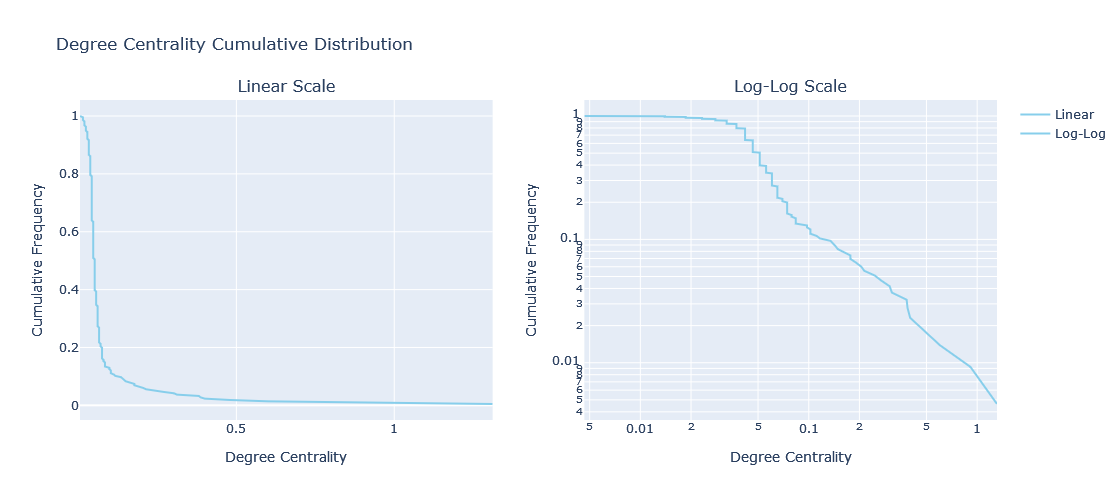
\includegraphics[width=.8\textwidth]{figures/question2/figure_5.png}
\captionsetup{font=scriptsize,labelfont=bf}
\caption{Cumulative Distribution for Degree Centrality.}
\label{fig:figure5}
\end{figure}

The huge steep suggests again that a few number of countries have high degree centrality, reinforcing the idea that the trade network may be dominated by a few powerful nations.

\subsubsection{Pagerank}
\textit{PageRank} is an alternative measure to eigenvector centrality that takes into account both the quantity and quality of incoming links. A high PageRank is given to those countries whose trading partners are themselves highly ranked. In other words, a country with a high PageRank has strong trade connections with other influential or well-connected countries, indicating that it is part of a network where it is linked to and valued by prominent players.

\begin{figure}[ht]
\centering
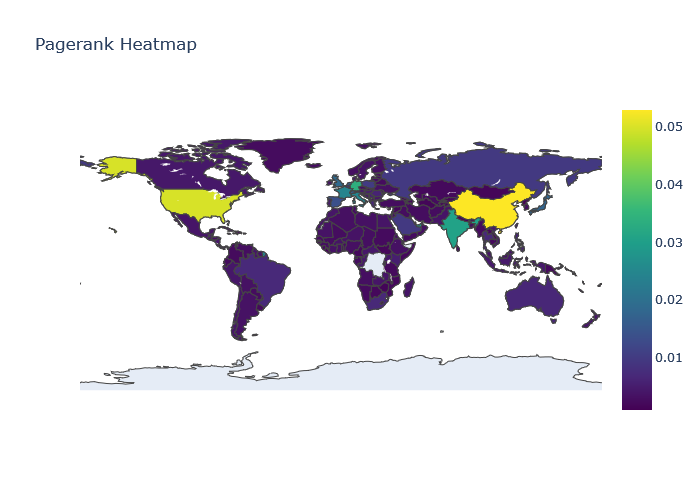
\includegraphics[width=.6\textwidth]{figures/question2/figure_6.png}
\captionsetup{font=scriptsize,labelfont=bf}
\caption{Pagerank heatmap.}
\label{fig:figure6}
\end{figure}

The observation of this geographic heatmap is particularly striking. It seems that countries renowned for their poverty are excluded from the trade routes that are instead maintained among significantly developed countries. \textbf{European countries}, \textbf{China}, \textbf{India} and the \textbf{United States} have the highest values.

\subsection{Is this group of strictly interconnected nations composed by wealthy states?}
\subsubsection{Pagerank}
We can take again into account the PageRank measure to have an highlight of the most influential countries in the network as long as the least influential ones. Then we can compare it to the GDP of each country to help us answering the question.

% \begin{figure}[!ht]
% \centering
% 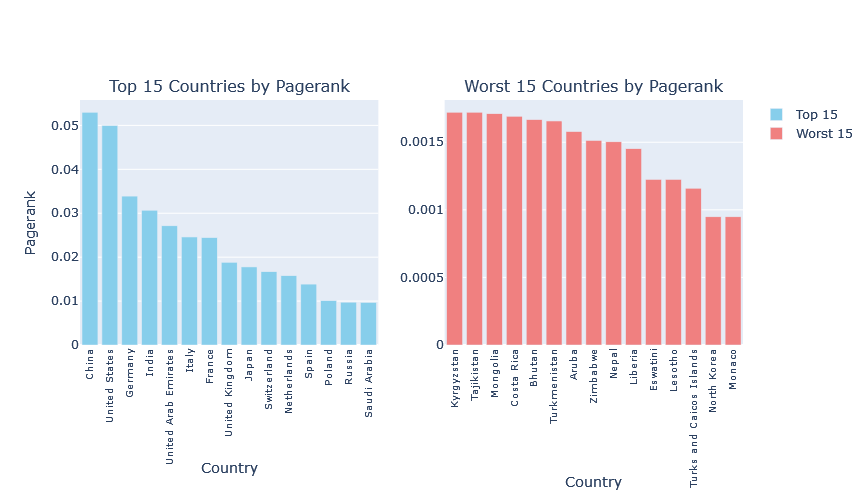
\includegraphics[width=.8\textwidth]{figures/question3/figure_7a.png}
% \vspace{1em}
% 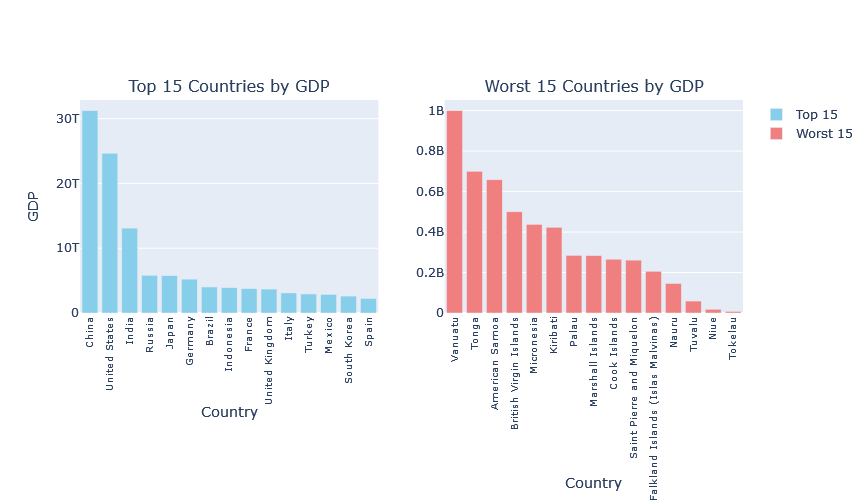
\includegraphics[width=.8\textwidth]{figures/question3/figure_7b.png}
% \captionsetup{font=scriptsize,labelfont=bf}
% \label{fig:figure7}
% \end{figure}

\begin{figure}[!ht]
\centering
\begin{minipage}[b]{0.49\textwidth}
    \centering
    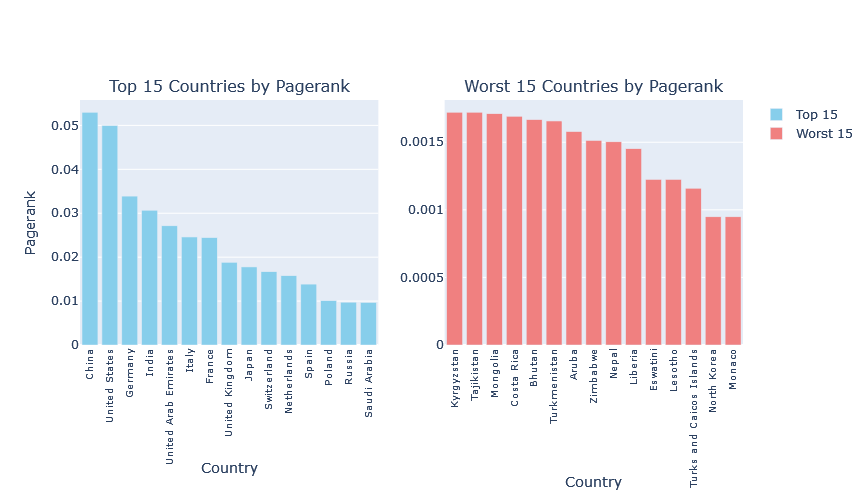
\includegraphics[width=\textwidth]{figures/question3/figure_7a.png}
\end{minipage}
\hfill
\begin{minipage}[b]{0.49\textwidth}
    \centering
    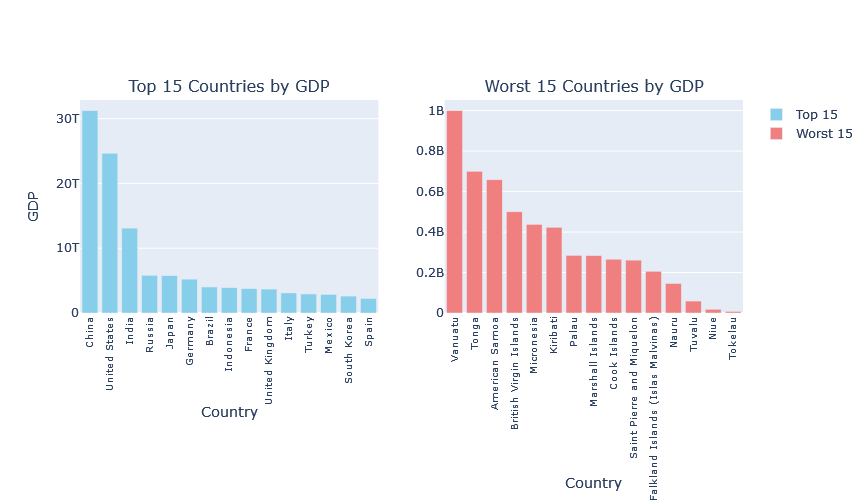
\includegraphics[width=\textwidth]{figures/question3/figure_7b.png}
\end{minipage}
\captionsetup{font=scriptsize,labelfont=bf}
\caption{Top and worst 10 countries by pagerank (left) and by GDP values (right).}
\label{fig:figure7}
\end{figure}

It's immediately visible a similar trend between the histograms: many of the same countries appear in the top ranks for both GDP and PageRank, such as the \textit{United States}, \textit{China}, \textit{Germany}, and \textit{India}. There is also a noticeable drop in both values after the top few countries; while a few countries are exceptionally dominant in both economic and network terms, the majority of nations in the top \textit{20} have significantly lower values, reflecting a sharp concentration of power and influence among the top global players.\\

We can further inspect this possible correlation by computing the \textit{Pearson Correlation Coefficient} between our values; it measures the linear relationship between two variables, and it can be applied to understand whether countries that are more central in the network according to their PageRank values also tend to have higher (or lower) GDPs.

\begin{figure}[!ht]
\centering
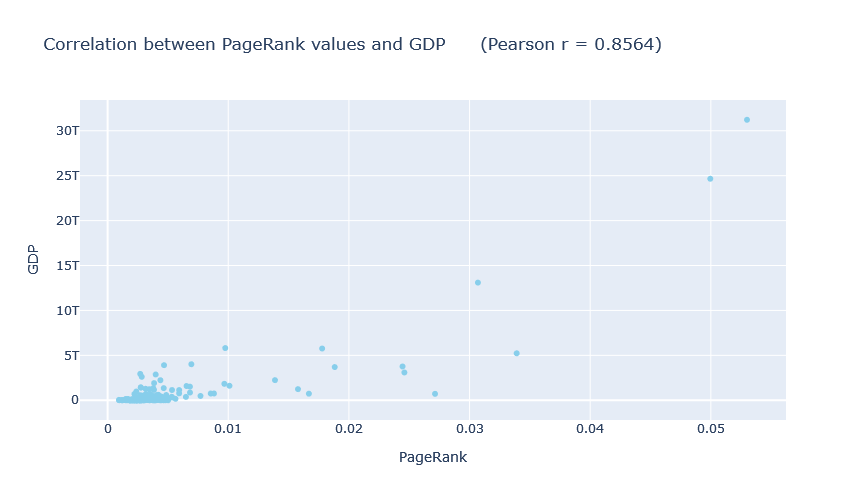
\includegraphics[width=.8\textwidth]{figures/question3/figure_8.png}
\vspace{1em}
\captionsetup{font=scriptsize,labelfont=bf}
\caption{Correlation between PageRank and GDP.}
\label{fig:figure8}
\end{figure}

The Pearson correlation coefficient is \textit{0.8564}, which is very close to \textit{1}, indicating a strong positive linear relationship between the PageRank values and GDP. The strength of the correlation suggests that the relationship between PageRank and GDP can be well-approximated by a linear model, where an increase in PageRank is associated with an increase in GDP.\\

The p-value is extremely small (p = \textit{2.2826e-63}), much smaller than the typical significance level of \textit{0.05}: the likelihood of observing such a strong correlation by random chance is virtually zero. In hypothesis testing, a small p-value allows us to reject the null hypothesis, which would typically state that there is no linear relationship between the two variables. Therefore, we can confidently say that there is a statistically significant correlation between PageRank values and GDP.\\

The distribution in the scatter plot furthermore validate the thesis. Most data points appear clustered towards the lower end of both PageRank and GDP, but a few countries with higher PageRank values also have higher GDPs, contributing to the strong positive correlation.

\subsection{What is the role of China and USA?}
\subsubsection{Hyperlink-Induced Topic Search (HITS)}

Although the other measures already stressed the unquestionable position of control assumed by these two countries, let us now assess their role. \textit{HITS} (\textit{Hyperlink-Induced Topic Search}) is an algorithm used to rank web pages based on their link structure, identifying \textit{hubs} (nodes linking to many other nodes) and \textit{authorities} (nodes that are linked to by many hubs). In our network, HITS would identify major exporters (hubs) and influential importers (authorities); the \textbf{USA} and \textbf{China} would likely emerge in both standings, highlighting their central roles.

\begin{figure}[!ht]
\centering
\begin{minipage}[b]{0.49\textwidth}
    \centering
    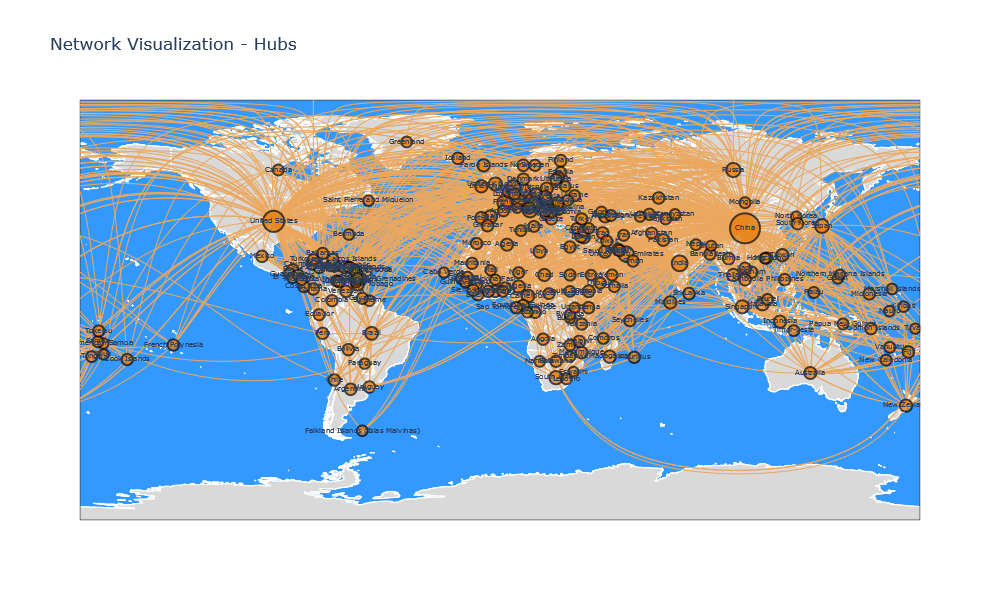
\includegraphics[width=\textwidth]{figures/question4/figure_9_h1.png}
\end{minipage}
\hfill
\begin{minipage}[b]{0.49\textwidth}
    \centering
    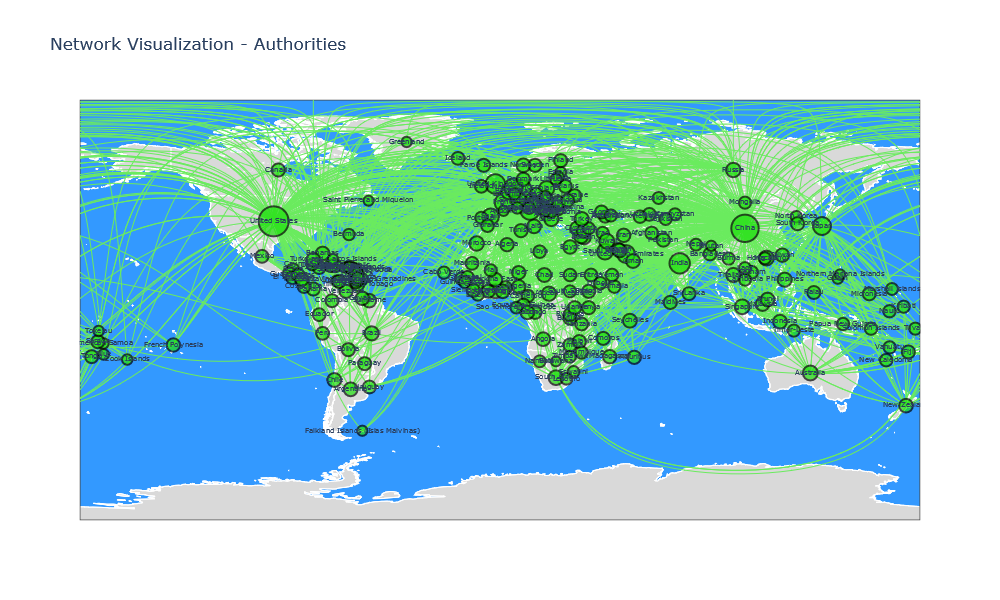
\includegraphics[width=\textwidth]{figures/question4/figure_9_a1.png}
\end{minipage}
\captionsetup{font=scriptsize,labelfont=bf}
\caption{HITS results. Node size proportional to hub value (left) and to authority value (right).}
\label{fig:figure9}
\end{figure}

From these plots, we mainly notice how \textit{China} corroborates its proficiency in exportation, while the \textit{United States} attests to its important role as a major authorithy for commodity traffic; it could be interesting to inspect what would happen if we remove both these countries.

\begin{figure}[!ht]
\centering
\begin{minipage}[b]{0.49\textwidth}
    \centering
    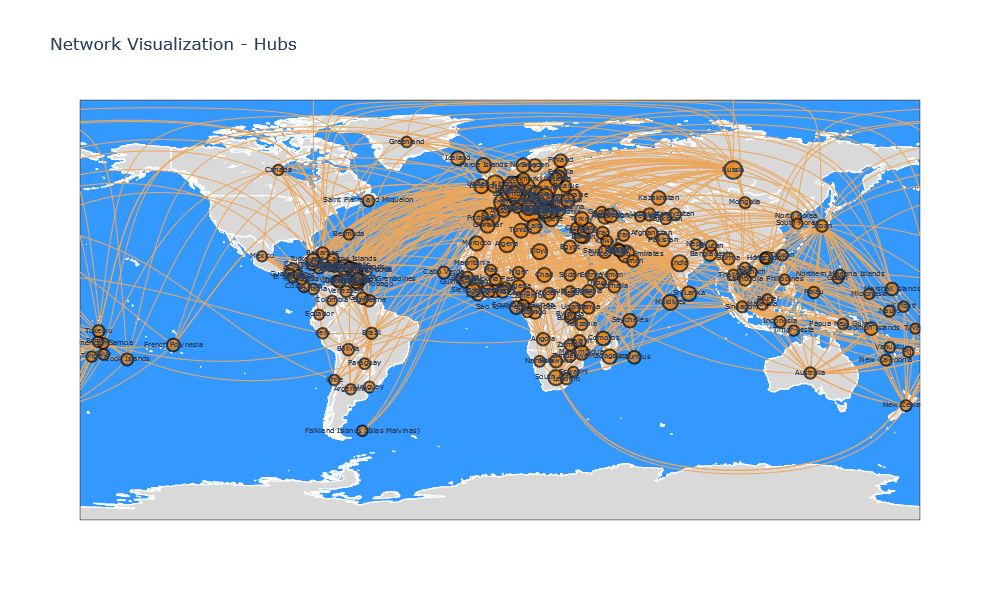
\includegraphics[width=\textwidth]{figures/question4/figure_10_h2.png}
\end{minipage}
\hfill
\begin{minipage}[b]{0.49\textwidth}
    \centering
    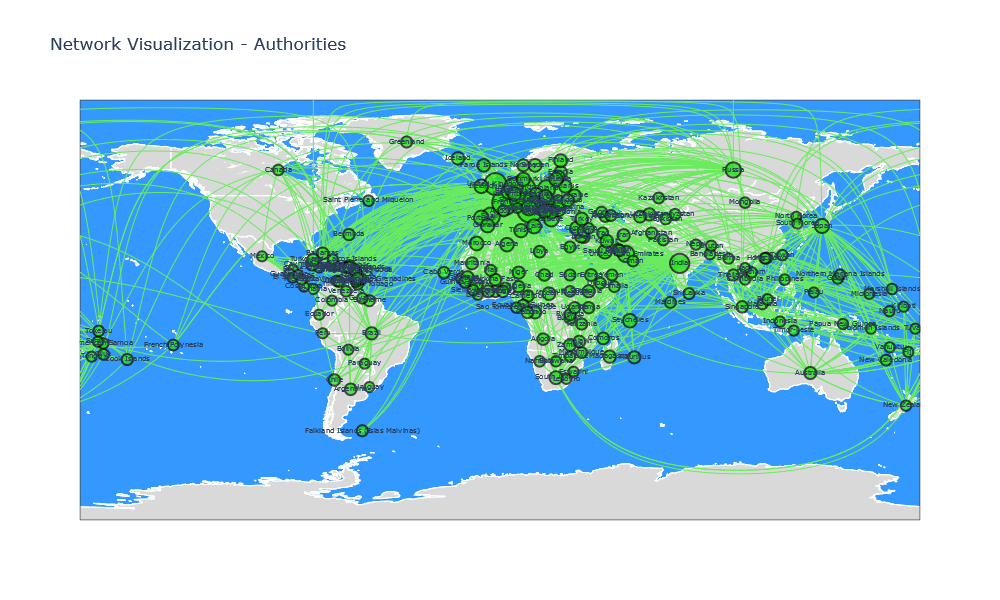
\includegraphics[width=\textwidth]{figures/question4/figure_10_a2.png}
\end{minipage}
\captionsetup{font=scriptsize,labelfont=bf}
\caption{HITS results after removing China and US. Node size proportional to hub value (left) and to authority value (right).}
\label{fig:figure9}
\end{figure}

The shift towards European countries is evident; the hubs (nodes connecting to many other nodes) experience significant growth, particularly among EU countries. On the other hand, the authorities (nodes that receive many links) show a general decrease for all countries except the European ones: this suggests that smaller countries were likely trading with the two superpowers, while relying on imports from other nations.

\subsubsection{SimRank}

\textit{SimRank} is a similarity metric that states, "two objects are considered to be similar if they are referenced by similar objects".
The pseudo-code definition from the paper is:
\begin{verbatim}
def simrank(G, u, v):
    in_neighbors_u = G.predecessors(u)
    in_neighbors_v = G.predecessors(v)
    scale = C / (len(in_neighbors_u) * len(in_neighbors_v))
    return scale * sum(
        simrank(G, w, x) for w, x in product(in_neighbors_u, in_neighbors_v)
    )
\end{verbatim}

Similarity in SimRank is measured by how alike two nodes are based on the similarity of their neighbors. In this network, a high SimRank score between two countries indicates that they trade with similar partners; however, the large number of partners that China has could potentially bias the results.

\begin{figure}[!ht]
\centering
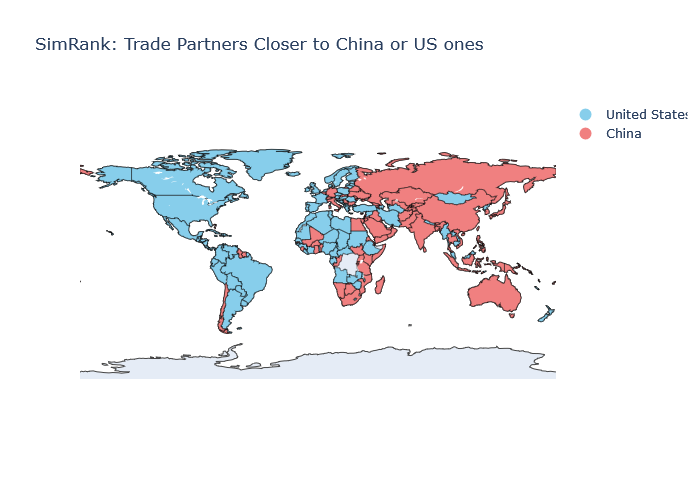
\includegraphics[width=.8\textwidth]{figures/question4/figure_11.png}
\vspace{1em}
\captionsetup{font=scriptsize,labelfont=bf}
\caption{Simrank plots, a country has either more trading partners in common with \textit{United States} or \textit{China}.}
\label{fig:figure11}
\end{figure}

As we observe, the countries looks almost splitted in half, with the left part labeled as \textit{United States} and the right part as \textit{China}; this behaviour is expected, since probably closer countries tend to trade with closer neighbours, leading the algorithm to split them territorially.

\subsubsection{Local Clustering Coefficient}

The \textit{Local Clustering Coefficient} measures the degree to which nodes in a graph tend to cluster together; it corresponds to the ratio between the connected pairs of neighbors of a node over all its neighbors pairs. A higher clustering coefficient could suggests that countries tend to trade more with their neighbors, forming tightly-knit clusters; we want to explore this measure to confirm our previously formulated hypotesis that this may be the reason why SimRank splits the world in half when looking for countries more similar either to \textit{China} or \textit{United States}.

\begin{figure}[!ht]
\centering
\begin{minipage}[b]{0.49\textwidth}
    \centering
    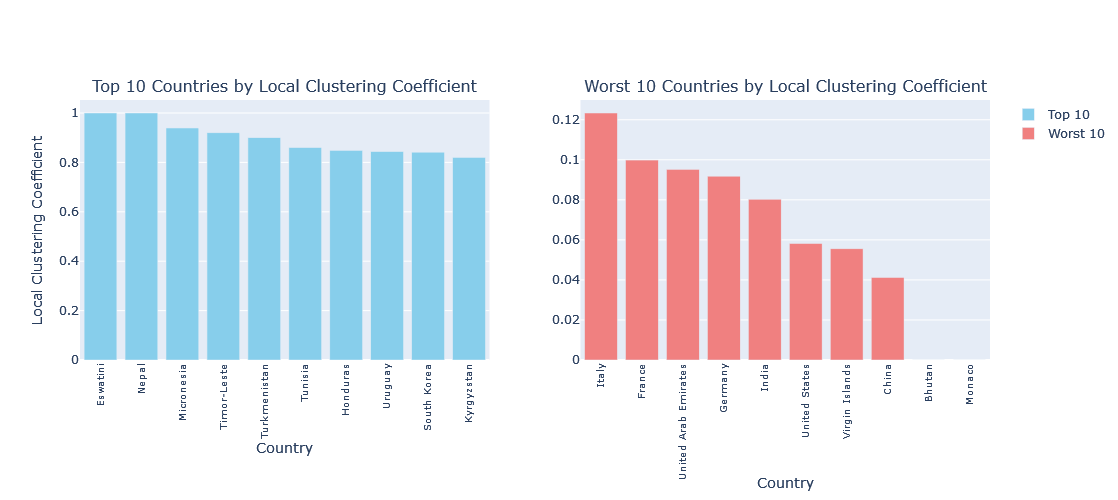
\includegraphics[width=\textwidth]{figures/question4/figure_12a.png}
\end{minipage}
\hfill
\begin{minipage}[b]{0.49\textwidth}
    \centering
    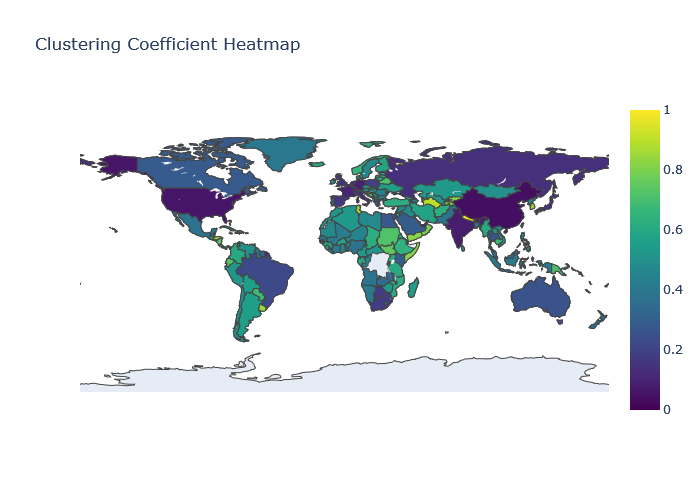
\includegraphics[width=\textwidth]{figures/question4/figure_12b.png}
\end{minipage}
\captionsetup{font=scriptsize,labelfont=bf}
\caption{Top and worst 10 countries by pagerank (left) and by GDP values (right).}
\label{fig:figure12}
\end{figure}














\section{Conclusion}
\label{conclusion}

The study's quantitative findings reveal significant insights into the structure of international trade. Key players identified through centrality measures are crucial for understanding global trade dynamics. The analysis highlights the importance of certain countries as major hubs, which can influence economic stability and policy making. These findings underscore the value of network analysis in economic studies.

\section{Critique}
\label{critique}

The work addresses the problem of understanding international trade networks to a significant extent by identifying key players and patterns. However, there are areas for improvement:

Data Quality: Gathering more detailed and up-to-date trade data could enhance the accuracy of the analysis.
Model Complexity: Incorporating additional factors such as trade volumes and economic indicators could provide a more comprehensive view.
Alternative Measures: Exploring other network measures or machine learning approaches could yield further insights.
Overall, the study provides a solid foundation for understanding international trade networks but could benefit from deeper and more nuanced analysis.

\end{document}